\documentclass{sig-alternate-10pt}
\usepackage{multirow, rotating, amsmath, wasysym}
\usepackage[tight]{subfigure}
\usepackage[ruled,linesnumbered,vlined]{algorithm2e}
\usepackage{hyperref}
\usepackage{color,soul}
\usepackage{array, graphicx}
\usepackage{epstopdf}
\usepackage{subfigure}
\usepackage{caption}

\graphicspath{{../}{figures/}}

\mathchardef\Gamma="0100 \mathchardef\Delta="0101
\mathchardef\Theta="0102 \mathchardef\Lambda="0103
\mathchardef\Xi="0104 \mathchardef\Pi="0105
\mathchardef\Sigma="0106 \mathchardef\Upsilon="0107
\mathchardef\Phi="0108 \mathchardef\Psi="0109
\mathchardef\Omega="010A

\newcommand{\ovspace}[1]{\vspace{#1}}

\newcommand{\outline}[1]{}%{\textbf{#1}}

\newcommand{\dl}{\mbox{$\, [ \hspace*{-1.5pt} [\,$}}
\newcommand{\dr}{\mbox{$\, ] \hspace*{-1.5pt} ]\:$}}
\newcommand{\da}{\mbox{$\, A \hspace*{-6.75pt} A \,$}}
%\newcommand{\drightarrow}{\mbox{$\rightarrow \hspace*{-8pt} \rightarrow$}}

\newcommand{\BA}{\mbox{${\bm{a}}$}}
%\newcommand{\BB}{\mbox{${\bm{c}}$}}
\newcommand{\BC}{\mbox{${\bm{c}}$}}
\newcommand{\BD}{\mbox{${\bm{d}}$}}
\newcommand{\BE}{\mbox{${\bm{e}}$}}
\newcommand{\BO}{\mbox{${\bm{o}}$}}
\newcommand{\BP}{\mbox{${\bm{p}}$}}
\newcommand{\BQ}{\mbox{${\bm{q}}$}}
\newcommand{\BR}{\mbox{${\bm{r}}$}}
\newcommand{\BV}{\mbox{${\bm{v}}$}}
\newcommand{\BL}{\mbox{${\bm{l}}$}}
\newcommand{\BI}{\mbox{${\bm{i}}$}}
\newcommand{\BH}{\mbox{${\bm{h}}$}}
\newcommand{\BS}{\mbox{${\bm{s}}$}}
\newcommand{\BB}{\mbox{${\bm{k}}$}}

\newcommand{\wrapbox}[1]{\framebox{\begin{tabular}{c}#1\end{tabular}}}
\newcommand{\CodeIn}[1]{{\small\texttt{#1}}}
\newcommand{\Section}[1]{Section~\ref{sec:#1}}
\newcommand{\SFigure}[2]{Figure~\ref{fig:#1}(#2)}

\usepackage{cite}
\usepackage{xspace}
\usepackage{url}
\usepackage{graphicx}
\usepackage{latexsym}
\usepackage{amssymb}
\usepackage{amsfonts}
%\usepackage{times}
\usepackage{psfrag}
%\usepackage{subfigure}
\usepackage{wrapfig}
\usepackage{comment}
%packages for algorithms
%\usepackage{algorithm}
%\usepackage{algorithmic}
\usepackage{alltt}
\usepackage{color}

\newtheorem{defn}{Definition}[section]
\newtheorem{exmp}{Example}[section]
\newtheorem{thrm}{Theorem}[section]
\newtheorem{prop}{Proposition}[section]
\newtheorem{lemm}{Lemma}[section]
\newtheorem{obsv}{Observation}[section]
\newtheorem{corr}{Corollary}[section]

%\addtolength{\textheight}{.23in} \addtolength{\textwidth}{.15in}
%\addtolength{\topmargin}{-.23in}
%\addtolength{\oddsidemargin}{.1in}
%\addtolength{\evensidemargin}{.1in}

\newtheorem{thm}{Theorem}
\newtheorem{dfn}{Definition}
\newtheorem{lem}{Lemma}
\newtheorem{cor}{Corollary}
\newcommand{\ie}{\emph{i.e.}\xspace}
\newcommand{\eg}{\emph{e.g.}\xspace}
\newcommand{\etc}{\emph{etc.}\xspace}
\newcommand{\etal}{\frenchspacing{}\emph{et al{.}}\xspace}
%\newcommand{\etal}[1]{{\sl et al.{#1}}}

%\newcommand{\thm}[1]{Theorem~\ref{thm:#1}}
%\newcommand{\lem}[1]{Lemma~\ref{lemma:#1}}
%\newcommand{cor}[1]{Corollary~\ref{cor:#1}}
\newcommand{\fac}[1]{Fact~\ref{fact:#1}}
\newcommand{\Table}[1]{Table~\ref{tab:#1}}
\newcommand{\Figure}[1]{Figure~\ref{fig:#1}}

%\theoremstyle{plain}
\newtheorem{property}{Property}[section]
\newtheorem{lemma}{Lemma}[section]
\newtheorem{corollary}{Corollary}[section]
\newtheorem{theorem}{Theorem}[section]

%\theoremstyle{definition}
\newtheorem{notation}{Notation}
\newtheorem{Definition}{Definition}[section]

%\theoremstyle{remark}
\newtheorem{fact}{Fact}[section]
\newtheorem{observation}{Observation}[section]
\newtheorem{insight}{Insight}[section]

%%\algorithmstyle{definition}
%\algsetup{indent=1em}
%\renewcommand{\algorithmicrequire}{\textbf{Input:  }}
%\renewcommand{\algorithmicensure}{\textbf{Output:}}
\newcommand{\factorial}{\ensuremath{\mbox{\sc Factorial}}}

\newcommand{\Comment}[1]{}

\renewcommand\floatpagefraction{0.999}
\renewcommand\topfraction{0.999}
\renewcommand\bottomfraction{0.999}
\renewcommand\textfraction{0.001}
\setcounter{totalnumber}{5}

\newcommand{\subfigs}{\hspace{-0.10in}}

\newcommand{\presec}{\vspace{0in}}
\newcommand{\postsec}{\vspace{0in}}
\newcommand{\presub}{\vspace{0in}}
\newcommand{\postsub}{\vspace{0in}}
\newcommand{\precaption}{\vspace{0in}}
\newcommand{\postcaption}{\vspace{0in}}
\newcommand{\preequation}{\vspace{0in}}
\newcommand{\postequation}{\vspace{0in}}
\newcommand{\prefig}{\vspace{0in}}
\newcommand{\prefigcaption}{\vspace{0in}}
\newcommand{\postfig}{\vspace{0in}}
\newcommand{\subfigsvert}{\vspace{0in}}
\newcommand{\pretheorem}{\vspace{0in}}
\newcommand{\posttheorem}{\vspace{0in}}


\newcommand{\Proc}{Proc. }
\newcommand{\Conf}{Conf. }
\newcommand{\Inte}{Int. }

\definecolor{pink}{rgb}{0.858, 0.188, 0.478}

\newcommand{\nan}[1]{\sethlcolor{pink}\hl{[Nan: #1]}}
\newcommand{\wei}[1]{\sethlcolor{green}\hl{Wei: #1}}
\newcommand{\judy}[1]{\sethlcolor{yellow}\hl{Judy: #1}}

\title{Learning to be Poetic:\\
Automatic Generation of Chinese Song Ci Using RNN}
\numberofauthors{3}
\author{
\alignauthor
Nan Du\\
	\affaddr{Michigan State University}\\
	\affaddr{East Lansing, MI 48823, USA}\\
	\email{dunan@msu.edu}
\alignauthor
Wei Wang\\
	\affaddr{Michigan State University}\\
	\affaddr{East Lansing, MI 48823, USA}\\
	\email{wangwe90@msu.edu}
\alignauthor
Zhuangdi Zhu\\
	\affaddr{Michigan State University}\\
	\affaddr{East Lansing, MI 48823, USA}\\
	\email{zhuzhuan@msu.edu}
}
% There's nothing stopping you putting the seventh, eighth, etc.
% author on the opening page (as the 'third row') but we ask,
% for aesthetic reasons that you place these 'additional authors'
% in the \additional authors block, viz.
\begin{document}
\maketitle


\sloppy
% !TEX root = /Users/zhuzhuangdi/Desktop/mobisys2017/main.tex
\begin{abstract}

In this paper, we study the side-channel information leakage from a laptop to a nearby mobile device.
%
Different from previous work that uses customized hardware to sense electromagnetic (EM) emissions,
%
we present  \emph{MagDetector}, which uses a mobile device to detect and recognize applications running on a laptop by exploiting EM side-channel information leakage from the laptop's CPU.
% 
To detect the launching of an application, we use two detection models based on machine learning techniques.
%
To recognize an launched application, we extract a time-variant feature vector for each application's EM signal based on short time fourier transform and principal component analysis.
%
After we recognize the launched application, we can even recognize different user operations inside the application based on wavelet multi-resolution analysis.  
%
 We implemented \emph{MagDetector} using a smartphone and evaluated it against 10 applications running on a MacBook laptop.
 %
\emph{MagDetector} detected the 10 applications with precision greater than 96\%, and recall greater than 93\%, respectively.
%
It classified the 10 applications with an average accuracy greater than 98\%.
 %
For user operation recognition, it classified 50 webpages opened in a web-browser with an average accuracy greater than 84\%.
 
 
\end{abstract}
\keywords{Side Channel Attack; Magnetometer; Commodity Mobile Device.}
\vspace{0.1in}
% !TEX root = /Users/zhuzhuangdi/Desktop/MSUCourses/MachineLearning847/17Project/17spr_wang_zhu_du/Proposal/main.tex
\section{Problem Description}
\subsection{Motivation}
In this project, we propose and evaluate different approaches to automatically generate Chinese poems. 
%
Especially, we study how to automatically generate Chinese Ci using machine learning skills.
%
Ci are one of the most important genres of Chinese classical poetry. 
%
As a precious cultural heritage, not many of them have been passed down onto the current generation.
%
Therefore, the study of automatic generation of Ci is meaningful, not only because it supplements entertainment and education resources to modern society, but also because it demonstrates the feasibility of applying artificial intelligence in Art generation. 
%

\subsection{Background}
Ci is a form of Chinese classical poetry. Arisen with the so-called banquet music in Tang dynasty. It reached its peak about hundred years later, and became a major alternative to Shi poetry\cite{cai2008chinesepoetry} in the Song dynasty.

Although different from even line structure used in Shi, Ci still follows strict rule determining the number of characters for different lines, the arrangement of rhyme, and the location of tones. There are more than 800 rule sets for Ci, which is called Cipai\cite{wikici}. The author of Ci needs to filling in the words according to the matrix associated to the Cipai. The uneven line used empower Ci to use more continuous syntax that traditional shi\cite{cai2008chinesepoetry}.

\subsection{Proposed Approach}
We propose an AI system which generate Ci in an interactive approach.
%
First, our system will prompt the user to provide a Cipai name.
%
Because Ci belonging to different Cipai may contain different emotions or grammatical rules.
%
Next, the system will receive few of keyword inputs that convey the detailed sentiments of the Song Ci.
%
the first sentence of the iambic will be generated based on the keyword inputs.
%
Further, the system generate following sentences based on previously-generated contexts using both RNN and SMT technique.
%
Finally, we evaluate the quality of the generated Ci using an evaluation tool named BLEU.

\subsection{Technical Challenges and Proposed Solutions}
The first challenge to build a general model for all types of Song Ci.
%
Different from Shi poetry whose structure is strict,  Song Ci has more than 800 set of Cipai, and different Cipai follows different structural or rhythmic patterns.
%
Therefore, it is difficult to generalize a model for all the Song Ci from limited training dataset.
% 
Our solution is to create a model based on Recurrent Neural Network. For every line generated in the SongCi, its probability is based on the probability of all previously lines.

Another challenge is to maintain consistent and poetic meanings throughout the generated SongCi.
%
Compared with Shi poetry, Song Ci are much longer in length and therefore more complicated in context.
%
It is difficult to keep long-distance memory using conventional RNN.
% 
Our solution is to use a Long Short Term Memory (LSTM) model that can track the long-distance information. 
\section{Related Work}  
% !TEX root = /Users/zhuzhuangdi/Desktop/MSUCourses/MachineLearning847/17Project/17spr_wang_zhu_du/Middle/middle_report.tex
\section{Methods}   
To automatically generate SongCi,  
First, we pre-process the SongCi corpus and tokenize each character.
%
Then we use a vector space model to convert each Chinese character in the corpus to be a vector presentation in the vector space so that characters with similar semantic meanings have small distance in the vector space.
%
Using the vector space as training data, we build a Recurrent Neural Network (RNN) that can generate SongCi with coherent and poetic meanings.
%
We add Long short-term memory (LSTM) units in our RNN model to capture long-term semantic dependencies in Song Ci.

\subsection{RNN}
%
%
RNNs are the family of the deep learning structures to process sequential data  \cite{rumelhart1986}. 
%
Parameter sharing across the different parts of the model is the key idea that makes RNNs to be able to deal with the sequential data. 
%
However, a simple RNNs cannot learn long time dependency as in the optimization this term tends to vanish or explode very fast \cite{goodfellow2016deeplearning}. 
%
To solve this challenge, gated RNNs is proposed and becomes one of the most effective practical models that used for sequential data.

\subsection{LSTM}
Long short-term memory (LSTM) model \cite{hochreiter1997lstm} is one branch of such gated RNNs that is extremely successful in the application like speech recognition, machine translation, and handwriting generation. 
%
The key idea of LSTM is to introduce a self loop so that gradient can flow for long duration. The self loop (internal recurrence) is located in "LSTM cells" with outer recurrence like ordinary recurrent network. The weight of self-loop is controlled by a forget gate \(f_i^{(t)}\)
:
\[f_i^{(t)} = \sigma (b_i^f + \sum_{j}U_{i,j}^f x_j^{(t)} +\sum_{j}W_{i,j}^f h_j^{(t-1)} ) \]
Where \(\boldsymbol{x}^{(t)}\) is the current input vector and \(\boldsymbol{h}^{(t)}\) is the current hidden layer vector, containing the outputs of all the LSTM cells. \(\boldsymbol{b}^f\), \(\boldsymbol{U}^f\), and \(\boldsymbol{W}^f\) are biases, input weights, and recurrent weights of the forget gate, respectively. The internal state of LSTM cell is updated with the following equation:
\begin{small}
\[s_i^{(t)} = f_i^{(t)}s_i^{(t-1)}+g_i^{(t)}\sigma(b_i + \sum_{j}U_{i,j}^f x_j^{(t)} +\sum_{j}W_{i,j}^f h_j^{(t-1)} )\]
\end{small}
And the external input gate unit 
\(g_i^{(t)} \)
is computed with the following equation:
\[g_i^{(t)} = \sigma (b_i^g + \sum_{j}U_{i,j}^g x_j^{(t)} +\sum_{j}W_{i,j}^g h_j^{(t-1)} ) \]
The output 
\(h^{(t)}\)
and the output gate 
\(q_i^{(t)}\)
, are updated using sigmoid function also:
\begin{eqnarray*}
h_i^{(t)} &=& \tanh (s_i^{(t)})q_i^{(t)}\\
q_i^{(t)} &=& \sigma (b_i^o + \sum_{j}U_{i,j}^o x_j^{(t)} +\sum_{j}W_{i,j}^o h_j^{(t-1)} )
\end{eqnarray*}

LSTM is proven to be able to learn long-term dependencies more effectively than normal RNNs. In our project, we will use LSTM as our main method. We also plan to compare LSTM performance with other network structures.
% !TEX root = /Users/zhuzhuangdi/Desktop/MSUCourses/MachineLearning847/17Project/17spr_wang_zhu_du/Middle/middle_report.tex
\section{Data Description}   
For our experiment, we obtained dataset for both Tang Shi and Song Ci. Many research were conducted for automatically generating Tang Shi. So we can evaluate our experiment result by comparing with these machine-created Tang Shi. And then we can move forward to Song Ci.
\subsubsection{Tang Poetry Corpus}
We use Quan Tangshi as our Tang Poetry corpus.\cite{1960quantangshi}. It was commissioned by Yin Cao in 1705 and published under the name of Kangxi Emperor. It contains 49,000 lyric poems (in the dataset we used it has 49,274 poems) and is believed the largest collection of Tang poetry. We obtained the dataset from the server of \cite{zhang2014chinese}.
\subsubsection{Song Ci Corpus}
% !TEX root = /Users/zhuzhuangdi/Desktop/MSUCourses/MachineLearning847/17Project/17spr_wang_zhu_du/Proposal/main.tex
\section{Proposal Summary and Project Milestones}
In this project, we aim at implementing an automatic Song Ci generator to generate Song Ci poems that can satisfy grammar, rhythmic and poetic requirements.
%
We implement this generator using two approaches. First, we will implement it using recurrent neural networks.
%
Next, we would like to implement it with using genetic algorithms.
%
We will compare the performance of different generating algorithms.
%
We plan to complete our project in the following four steps:
and detailed project timeline is showed in Figure \ref{fig:projecttimeline}:
\begin{figure}[htbp]
	\centering
	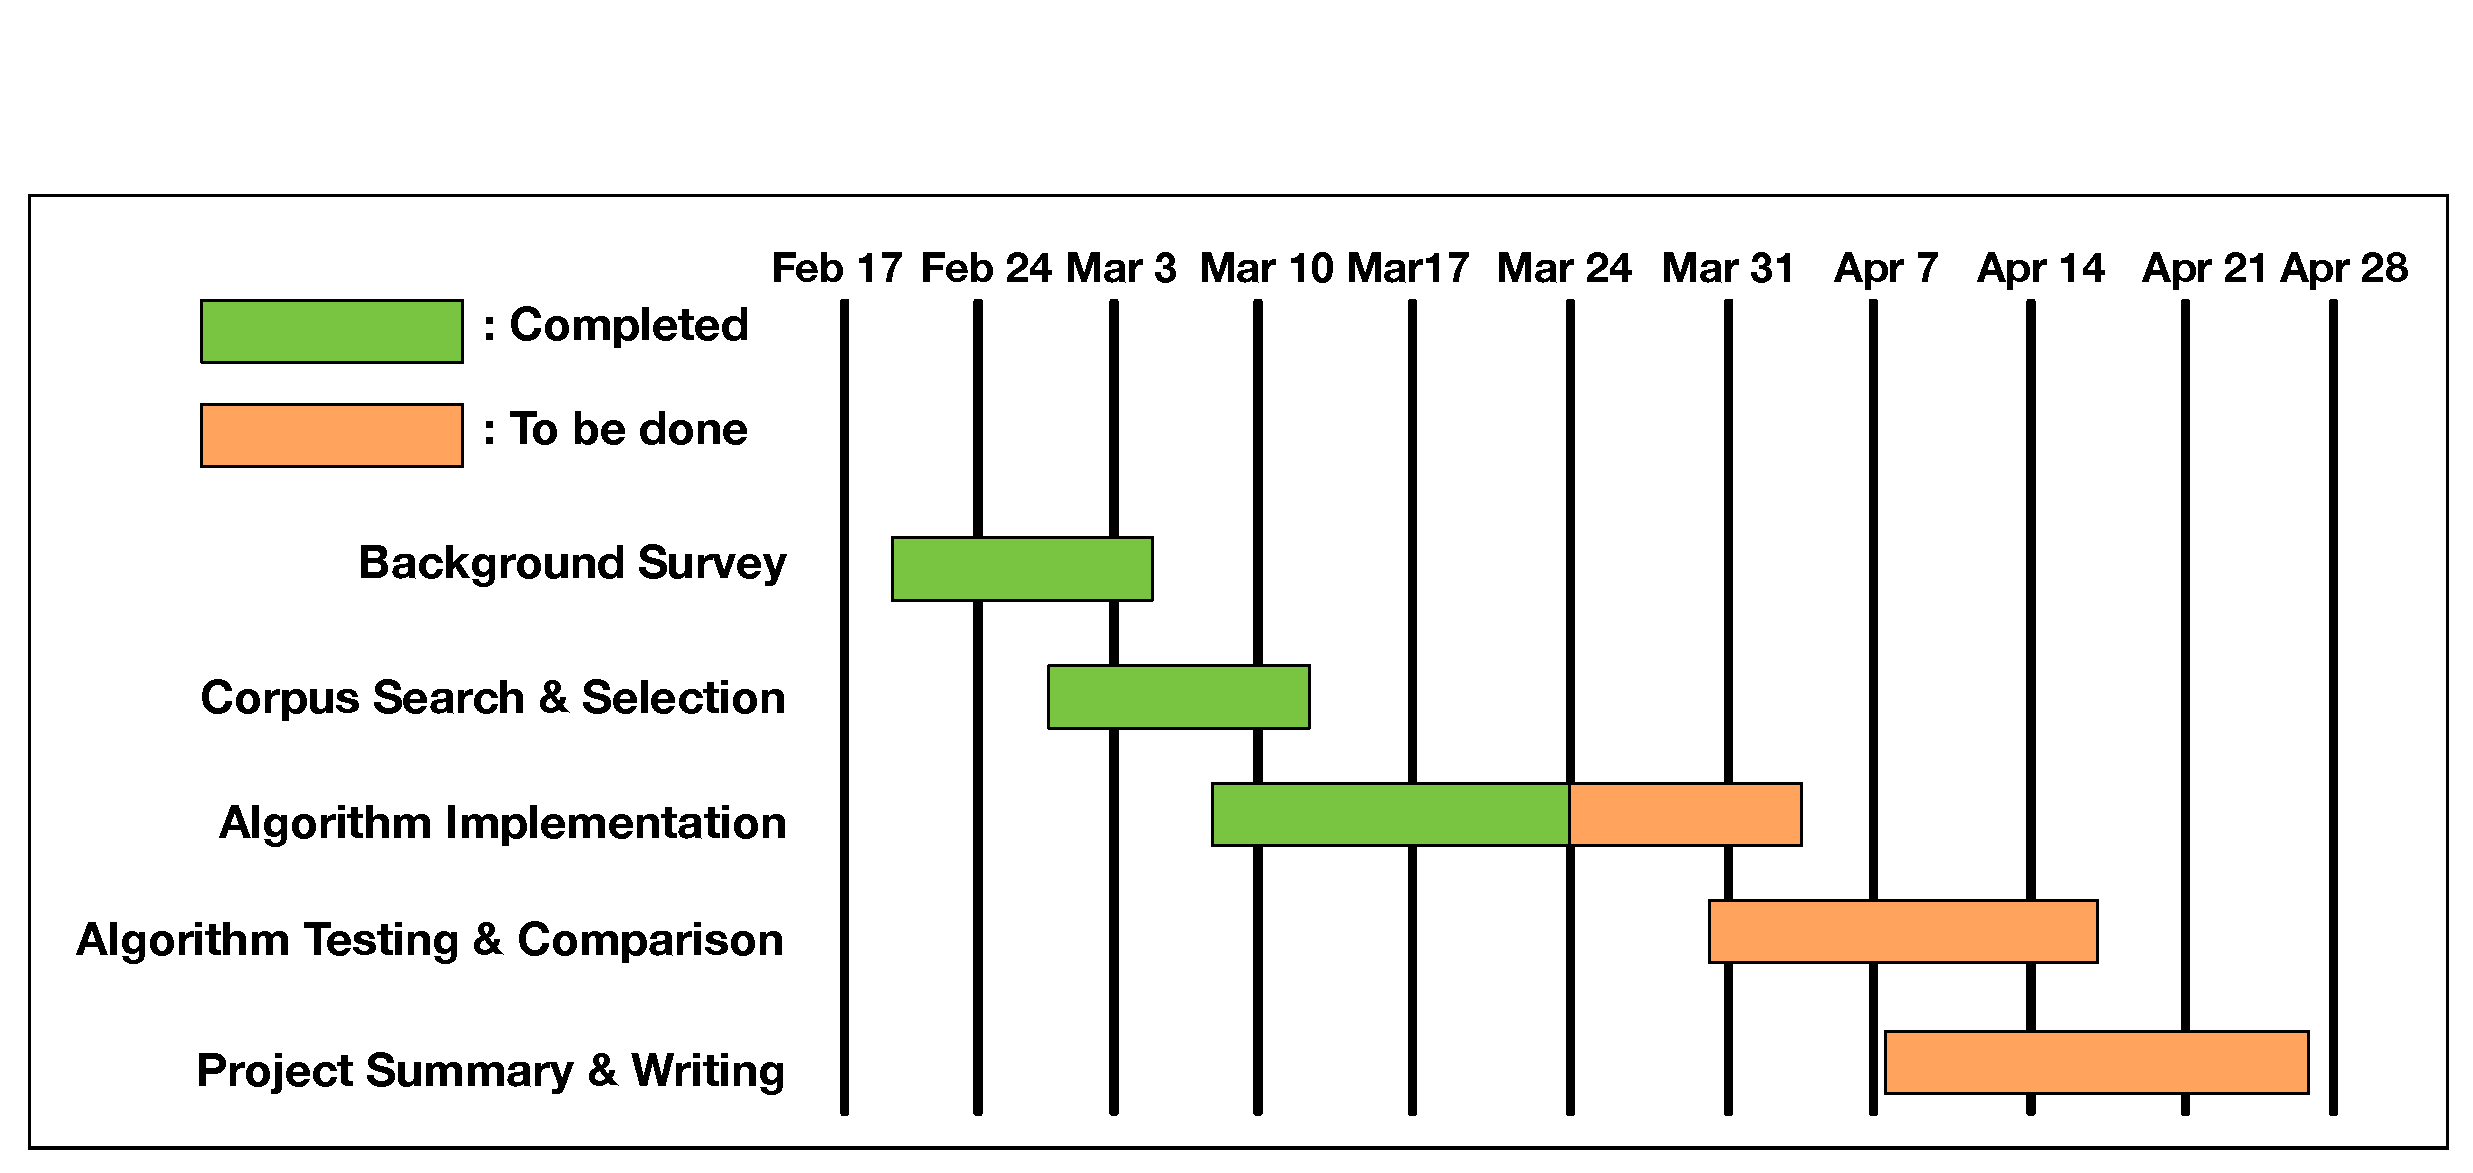
\includegraphics[width=0.9\linewidth]{mileStone}
	\caption{Project Timeline}
	\label{fig:projecttimeline}	
\end{figure}
\begin{itemize}
\item Background Survey
\item Corpus Search and Selection
\item Algorithm Implementation
\item Algorithm Testing and Comparison
\item Project Summary and Writing
\end{itemize}

For this initial step, we plan to search for related works to computational literary creation to gain the basic knowledge of Song Ci.
%
We are interested in the following questions: what is the criterion of a good Song Ci? How to evaluate the correctness, fluency and style of poems generated?
%
Better understanding of related work and Song Ci composition rules will provide us with great help for the following work, especially algorithm testing and comparison. 
%
Second, we will search and select a proper Song poem corpus for our project. The ideal corpus should be comprehensive on poem styles, and are precisely analyzed for content. 
%
Third, implementation poem generator based on both algorithm of RNN and genetic algorithm would be the most important work in our project. So we will assign more time on this step. 
%
Firth, test cases will be generated with both poem generator under the same keywords and topics. Poems will be test on aspects of grammar, semantic correctness, style and content. Both computational evaluation and human evaluation are expected to be used in last part of our project.



\bibliographystyle{abbrv}
\bibliography{middle_report}
\end{document}
